\chapter{Extensión analítica de COBRIA}

La analítica y la inteligencia artificial suelen incorporarse después de que un sistema
operacional ha acumulado datos. En ese momento aparecen exportaciones manuales,
significados incompatibles, atributos sin procedencia y modelos difíciles de reproducir.
COBRIA aborda este problema desde la arquitectura: considera conjuntos de datos, características,
embeddings, índices de recuperación y predicciones como proyecciones gobernadas de datos
canónicos y eventos autorizados.

La propuesta no convierte el dominio en un sistema de aprendizaje automático. Mantiene
una frontera explícita entre hechos de negocio, evidencia derivada e inferencias
probabilísticas. Esta frontera permite utilizar la misma disciplina de identidad, ámbito,
versionado, reconstrucción y trazabilidad tanto en minería descriptiva como en modelos
predictivos, recuperación aumentada y agentes.

\section{De la operación al conocimiento}

Se distinguen cinco niveles semánticos:

\begin{enumerate}[leftmargin=*]
  \item \textbf{Hecho canónico:} estado validado por un caso de uso y sujeto a
  invariantes del dominio.
  \item \textbf{Evento:} observación temporal de un cambio o interacción, con tiempo,
  ámbito y procedencia.
  \item \textbf{Derivación analítica:} transformación determinista o controlada, como
  una característica, agregado o fragmento.
  \item \textbf{Inferencia:} salida probabilística de un modelo, acompañada de versión,
  evidencia y medidas de incertidumbre disponibles.
  \item \textbf{Decisión:} acción aceptada por una persona o caso de uso autorizado.
\end{enumerate}

Una inferencia no asciende automáticamente a hecho. Si una clasificación, recomendación
o respuesta debe modificar el negocio, se formula como propuesta y atraviesa validación,
autorización e idempotencia. Esta regla evita que una salida plausible pero incorrecta
sobrescriba la fuente canónica.

\section{Capacidades analíticas}

\begin{table}[H]
\centering
\caption{Adaptación de COBRIA a modalidades analíticas.}
\label{tab:capacidades-analiticas}
\begin{tabularx}{\textwidth}{p{3.2cm}p{4cm}X}
\toprule
Modalidad & Proyección principal & Requisitos COBRIA \\
\midrule
Descriptiva & Agregado o cubo & Definición, ventana, ámbito y reconciliación.\\
Minería de datos & Conjunto de datos versionado & Semilla, filtros, linaje y calidad.\\
Series temporales & Secuencia por entidad & Tiempo de evento, ingestión y marca de corte.\\
Aprendizaje supervisado & Conjunto de características y etiquetas & Corte temporal y prevención de fuga.\\
Texto y multimedia & Fragmentos y descriptores & Resumen criptográfico, derechos, modelo extractor y versión.\\
Búsqueda semántica & Índice de embeddings & Modelo compatible, permisos y reconstrucción.\\
RAG & Corpus recuperable & Evidencia, vigencia y autorización previa.\\
Agentes & Herramientas tipadas & Capacidades mínimas, aprobación y auditoría.\\
\bottomrule
\end{tabularx}
\end{table}

\section{Componentes de la extensión}

La extensión de inteligencia se compone de un Constructor de conjuntos de datos, un Registro de características, un
Almacén de artefactos, un Registro de modelos, un Pasarela de recuperación, un Motor de políticas y un Evidencia
Registro. Estos componentes se apoyan en Núcleo, Metadatos, Proyecciones y Gobierno; no
acceden a rutas físicas mediante convenciones privadas.

\begin{figure}[H]
\centering
\begin{tikzpicture}[
  node distance=.7cm and .8cm,
  box/.style={draw,align=center,minimum width=2.4cm,minimum height=.82cm},
  derived/.style={box,fill=cobriaLight},
  line/.style={-{Latex[length=2mm]},thick}
]
\node[box] (core) {Núcleo y\\eventos};
\node[derived,right=of core] (datosNodo) {Constructor de\\conjuntos de datos};
\node[derived,right=of datosNodo] (características) {Registro de\\características};
\node[derived,below=of características] (models) {Registro de\\modelos};
\node[derived,left=of models] (retrieval) {Pasarela de\\recuperación};
\node[box,left=of retrieval] (usecase) {Caso de uso\\autorizado};
\node[box,below=of datosNodo] (policy) {Motor de políticas y Registro de evidencias};
\draw[line] (core) -- (datosNodo);
\draw[line] (datosNodo) -- (características);
\draw[line] (características) -- (models);
\draw[line] (models) -- (retrieval);
\draw[line] (retrieval) -- (usecase);
\draw[line,dashed] (policy) -- (datosNodo);
\draw[line,dashed] (policy) -- (models);
\draw[line,dashed] (policy) -- (retrieval);
\end{tikzpicture}
\caption{Componentes de la extensión analítica e inteligente de COBRIA.}
\label{fig:extension-inteligencia}
\end{figure}

\section{Principios de adaptación}

La extensión conserva ocho principios: autoridad canónica, derivación declarada,
reconstruibilidad proporcional, aislamiento por ámbito, corrección temporal, mínimo dato
necesario, evidencia enlazable y supervisión proporcional al riesgo. La
reconstruibilidad es proporcional porque no toda salida probabilística puede reproducirse
bit a bit; en esos casos se exige reproducibilidad del proceso, captura de parámetros y
medición de variación.

\chapter{Contratos de conjuntos de datos y linaje}

\section{Definición formal}

Un contrato de conjunto de datos se representa como:

\begin{equation}
\mathcal{D}=\langle id,v,Q,F,W,S,L,P,V,C\rangle,
\end{equation}

donde $id$ es la identidad; $v$, la versión; $Q$, la selección de fuentes; $F$, las
transformaciones; $W$, la política temporal o marca de corte; $S$, el esquema de salida;
$L$, el conjunto de etiquetas; $P$, las políticas; $V$, las validaciones; y $C$, las
condiciones de publicación. Una ejecución produce un manifiesto $M$ con entradas,
salidas, resúmenes criptográficos, tiempos, código y entorno.

El conjunto de datos se considera reconstruible si existen fuentes permitidas suficientes, las
transformaciones y dependencias están fijadas, el contrato puede ejecutarse y el
resultado puede verificarse según una equivalencia declarada. Para datos tabulares
deterministas puede exigirse igualdad exacta; para conversiones multimedia o librerías
no deterministas se requiere tolerancia documentada.

\section{Contrato mínimo}

\begin{longtable}{>{\bfseries}p{3.2cm}p{5.1cm}p{6cm}}
\caption{Contenido mínimo de un contrato de conjunto de datos.}\label{tab:contrato-conjunto de datos}\\
\toprule
Elemento & Pregunta que responde & Evidencia conservada \\
\midrule
\endfirsthead
\toprule
Elemento & Pregunta que responde & Evidencia conservada \\
\midrule
\endhead
Propósito & ¿Para qué análisis puede utilizarse? & Tarea, población y usos excluidos.\\
Fuentes & ¿De dónde procede cada campo? & Tipo canónico, evento, versión y ámbito.\\
Selección & ¿Qué se incluye o excluye? & Predicados, ventanas y razones.\\
Transformación & ¿Cómo se obtiene cada variable? & Función, parámetros y código.\\
Tiempo & ¿Qué era conocido en el corte? & tiempo del evento, tiempo de ingestión y marca de corte.\\
Esquema & ¿Qué significa cada columna? & Tipo, unidad, dominio y nulabilidad.\\
Calidad & ¿Qué condiciones debe cumplir? & Reglas, umbrales y resultados.\\
Privacidad & ¿Qué datos están permitidos? & Base de acceso, minimización y retención.\\
Publicación & ¿Cuándo es utilizable? & Aprobación, hash, ubicación y estado.\\
Retiro & ¿Cuándo deja de utilizarse? & Fecha, motivo y dependencias notificadas.\\
\bottomrule
\end{longtable}

Este contrato complementa prácticas de documentación como las fichas de datos, que
buscan explicitar motivación, composición, proceso de recolección, usos y mantenimiento
\parencite{gebru2021datasheets}. COBRIA añade correspondencia ejecutable con entidades,
proyecciones y ámbitos del sistema.

\section{Grafo de linaje}

El linaje se modela como un grafo dirigido acíclico $G_L=(V_L,E_L)$. Los nodos pueden
ser fuentes, ejecuciones, conjuntos de datos, características, modelos, evaluaciones y
predicciones. Una arista expresa \emph{derivado de}, \emph{entrenado con},
\emph{evaluado con} o \emph{producido por}. Cada nodo posee identidad y versión; una etiqueta textual
sin referencia estable no constituye linaje suficiente.

Para una predicción $y$, la consulta de procedencia debe poder recorrer:

\begin{equation}
y\rightarrow \text{modelo}\rightarrow \text{Conjunto de características}\rightarrow
\text{conjunto de datos}\rightarrow \text{fuente canónica o evento}.
\end{equation}

El grafo no almacena necesariamente los datos completos. Puede conservar resúmenes criptográficos,
manifiestos y referencias protegidas. Los permisos se vuelven a comprobar al navegar;
poseer el ID de un nodo no concede acceso a su contenido.

\section{Algoritmo de materialización}

\begin{verbatim}
BuildDataset(contractId, version, ámbito, cutoff):
  contract <- registry.require(contractId, version)
  policy.require("conjunto de datos.build", ámbito, contract.purpose)
  snapshot <- resolveSources(contract.sources, ámbito, cutoff)
  run <- ledger.start(contract, snapshot, actor, environment)
  for batch in snapshot.readBatches():
      rows <- contract.transform(batch)
      contract.validate(rows)
      artifact.write(run.stagingVersion, rows)
      run.checkpoint(batch.cursor, rows.hash)
  summary <- verify(run.stagingVersion, contract)
  if not summary.accepted: quarantine(run, summary)
  else publishAtomically(run, summary)
  return run.manifiesto
\end{verbatim}

La publicación se realiza después de validar, no mientras el conjunto de datos está incompleto.
Una ejecución fallida queda en cuarentena con sus métricas y no reemplaza la versión
vigente.

\section{Calidad y observabilidad}

Las reglas se agrupan en esquema, completitud, dominio, unicidad, integridad referencial,
distribución, tiempo y privacidad. Un cambio estadístico no siempre es un defecto; puede
reflejar un cambio real. Por eso las alertas de deriva generan revisión y no corrección
automática del canónico.

\chapter{Almacén de características, series temporales y minería de datos}

\section{Características como proyecciones}

Una característica se define mediante:

\begin{equation}
\phi=\langle nombre,v,entidad,ambito,tipo,unidad,g,W,frescura,responsable\rangle.
\end{equation}

La función $g$ transforma fuentes autorizadas; $W$ define la ventana temporal. La
identidad de entidad permite unir valores sin depender de campos ambiguos. El registro
describe significado y versión; los valores pueden almacenarse fuera de línea, en línea o en
ambos medios.

Los Almacenes de características buscan coordinar cálculo, almacenamiento y servicio de
características entre entrenamiento e inferencia \parencite{orr2021featurestores,
li2023featurestore}. COBRIA los incorpora como una especialización de sus proyecciones:
la definición vive en metadatos, la fuente conserva autoridad y las materializaciones
pueden reconstruirse.

\section{Equivalencia fuera de línea--en línea}

Sea $\phi_o(e,t)$ la característica calculada fuera de línea y $\phi_n(e,t)$ la servida en línea.
Se exige una relación de equivalencia:

\begin{equation}
\phi_o(e,t)\simeq_{\epsilon}\phi_n(e,t),
\end{equation}

donde $\epsilon=0$ para valores deterministas exactos y puede ser una tolerancia
justificada para cómputo numérico. Las diferencias se investigan por contrato, versión,
marca de corte, ventana y código. Compartir nombre no demuestra equivalencia.

\section{Corrección punto-en-tiempo}

Para una observación de entrenamiento en $t_c$, COBRIA solo admite una fuente $x$ si su
tiempo de disponibilidad satisface $t_a(x)\leq t_c$. El tiempo del evento puede ser
anterior y el de ingestión posterior; usar únicamente event time puede introducir
información que todavía no estaba disponible.

\begin{equation}
\mathcal{D}(t_c)=\{x\mid \operatorname{ambito}(x)=s\land t_a(x)\leq t_c\land
\operatorname{politica}(x)=\mathrm{permitido}\}.
\end{equation}

Esta condición reduce fuga temporal. Las etiquetas usan una ventana futura separada y
no participan en la construcción de características del mismo corte.

\begin{figure}[H]\centering
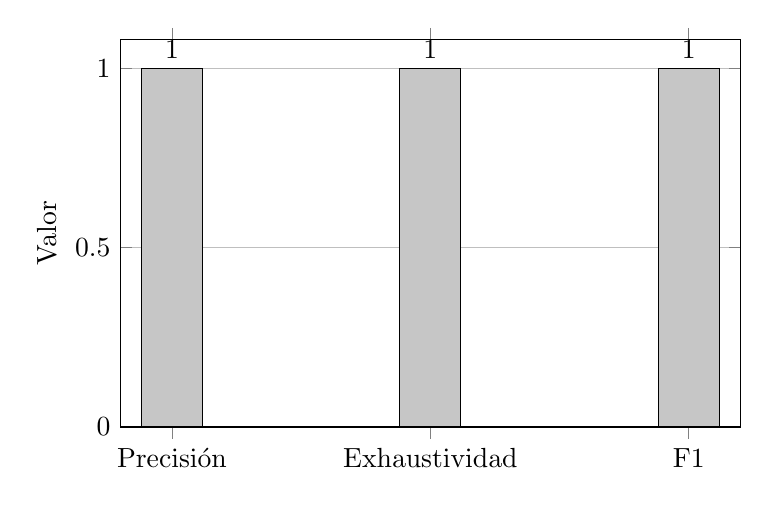
\begin{tikzpicture}\begin{axis}[ybar,bar width=22pt,width=.78\textwidth,height=6.5cm,ymin=0,ymax=1.08,ylabel={Valor},symbolic x coords={Precisión,Exhaustividad,F1},xtick=data,ymajorgrids=true,nodes near coords]
\addplot[fill=gray!45,draw=black] coordinates {(Precisión,1.0) (Exhaustividad,1.0) (F1,1.0)};\end{axis}\end{tikzpicture}
\caption{Contratos sintéticos de recuperación en 30 repeticiones. No constituyen evaluación humana de un modelo generativo.}\label{fig:contratos-ia}\end{figure}


\section{Eventos tardíos y marcas de avance temporal}

Los eventos se clasifican como a tiempo, tardíos pero aceptables, o fuera de la ventana
de corrección. La política declara cuánto se espera, cuándo se recalcula una proyección
y cuándo se publica una corrección. Un marca de corte no significa que nunca aparecerá otro
evento; expresa una decisión operacional sobre completitud suficiente.

\section{Minería descriptiva y descubrimiento}

COBRIA facilita segmentación, reglas de asociación, detección de anomalías y análisis de
secuencias porque cada observación conserva entidad, ámbito, tiempo y procedencia. El
proceso exploratorio puede descubrir nuevas variables o patrones, pero sus resultados
se registran como hipótesis analíticas. Una agrupación no redefine automáticamente una
categoría del negocio y una anomalía no implica fraude o error.

Para análisis no supervisado se versionan preprocesamiento, escalamiento, imputación,
selección de variables, métrica de distancia, algoritmo y semilla. Esto permite separar
la inestabilidad del algoritmo de cambios en los datos de entrada.

\section{Catálogo analítico}
\enlargethispage{3\baselineskip}

El catálogo enlaza entidades, eventos, características, conjuntos de datos, modelos y responsables.
Debe responder quién puede usar un artefacto, con qué propósito, de qué versión depende,
cuándo fue actualizado, qué calidad alcanzó y qué consumidores se verán afectados por
un cambio. No es solo una lista de archivos: refleja relaciones ejecutables del grafo de
linaje.

\chapter{Multimodalidad, embeddings y búsqueda semántica}

\section{Objeto multimedia canónico}

El canónico de un recurso multimedia no contiene necesariamente los bytes. Conserva
identidad, ámbito, propietario, tipo MIME validado, tamaño, hash, ubicación lógica,
tiempos, consentimiento o base de uso, retención y estado. Las miniaturas,
transcripciones, descriptores y embeddings son derivados.

Separar contenido y metadatos evita transportar objetos grandes en consultas comunes y
permite políticas distintas. Una URL temporal no es identidad permanente; el Artefacto
Pasarela resuelve la referencia solo después de autorización.

\section{Pipeline multimodal}

\begin{figure}[H]
\centering
\begin{tikzpicture}[
  node distance=.75cm and .8cm,
  box/.style={draw,align=center,minimum width=2.25cm,minimum height=.82cm},
  derived/.style={box,fill=cobriaLight},
  line/.style={-{Latex[length=2mm]},thick}
]
\node[box] (asset) {Recurso y\\metadatos};
\node[derived,right=of asset] (extract) {Extractor\\versionado};
\node[derived,right=of extract] (chunks) {Fragmentos /\\descriptores};
\node[derived,below=of chunks] (embed) {Modelo de\\embedding};
\node[derived,left=of embed] (index) {Índice\\semántico};
\node[box,left=of index] (retrieve) {Recuperación\\autorizada};
\draw[line] (asset) -- (extract);
\draw[line] (extract) -- (chunks);
\draw[line] (chunks) -- (embed);
\draw[line] (embed) -- (index);
\draw[line] (index) -- (retrieve);
\end{tikzpicture}
\caption{Pipeline multimodal reconstruible.}
\label{fig:pipeline-multimodal}
\end{figure}

Cada etapa genera un manifiesto. Para una transcripción se conserva idioma, modelo,
parámetros y segmentos temporales; para imagen, regiones o descriptores; para video,
fotogramas o intervalos; para series, frecuencia y método de remuestreo. Los errores de
extracción no modifican el recurso fuente.

\section{Contrato de embedding}

Un embedding se representa como:

\begin{equation}
\begin{aligned}
z=\langle &sourceId,sourceVersion,chunkId,modelId,\\
           &modelVersion,d,normalization,vector,policy\rangle.
\end{aligned}
\end{equation}

La dimensión $d$, normalización y modelo determinan compatibilidad. Dos vectores con la
misma dimensión no son necesariamente comparables. Una migración crea un índice nuevo,
recalcula y valida recuperación antes del cambio de versión.

Los modelos basados en atención permiten representar dependencias contextuales y son la
base de numerosos modelos modernos de lenguaje y modalidades relacionadas
\parencite{vaswani2017attention}. COBRIA no depende de una arquitectura de modelo
específica; registra qué modelo produjo cada representación.

\section{Fragmentación}

El contrato de fragmentación declara unidad, solapamiento, límites semánticos, tamaño
máximo y tratamiento de tablas o marcas temporales. Un fragmento mantiene referencia a
la fuente y desplazamientos suficientes para mostrar evidencia. Si cambia el documento, los
fragmentos anteriores quedan asociados a su versión y se generan otros nuevos.

Fragmentos demasiado pequeños pierden contexto; demasiado grandes disminuyen precisión
de recuperación y aumentan costo de instrucción. La elección se evalúa por corpus y tarea,
no mediante una constante universal.

\section{Recuperación híbrida}

La búsqueda puede combinar filtros estructurados, texto y similitud vectorial. Primero
se limita por ámbito, permiso, vigencia y tipo; después se puntúa. Aplicar autorización
solo al final permite que un documento prohibido influya en ranking o contexto.

\begin{equation}
score(x,q)=\alpha s_{vector}+\beta s_{text}+\gamma s_{metadata},
\end{equation}

con pesos versionados. El resultado incluye score por componente, modelo, consulta
normalizada y referencias. El score ordena candidatos; no prueba verdad.

\section{Derecho a retirar y reconstrucción}

Cuando un recurso se retira, se invalidan fragmentos, embeddings, cachés y conjuntos de datos que
lo contienen según la política. El grafo de linaje permite localizar dependencias. Un
modelo ya entrenado plantea un problema diferente: puede requerir evaluación, nuevo
entrenamiento o documentación de la limitación, según obligación y riesgo. Borrar una
fila del índice no demuestra que toda influencia desapareció.

\chapter{Recuperación aumentada y agentes gobernados}

\section{RAG como composición de proyecciones}

La recuperación aumentada combina una memoria paramétrica con evidencia recuperada para
producir respuestas condicionadas por fuentes externas \parencite{lewis2020rag}. En
COBRIA, el corpus, los fragmentos y el índice son proyecciones; la respuesta es una
inferencia; las entidades y documentos autorizados conservan autoridad.

Una ejecución se formaliza como:

\begin{equation}
r=\operatorname{Generar}(M_v,p,\operatorname{Recuperar}(I_v,q,ambito,politica),\theta),
\end{equation}

donde $M_v$ es el modelo, $p$ la plantilla, $I_v$ el índice, $q$ la consulta y $\theta$
los parámetros. El registro conserva todas estas versiones junto con fragmentos
recuperados, scores, filtros, tiempos y resultado.

\section{Flujo seguro de recuperación}

\begin{enumerate}[leftmargin=*]
  \item autenticar actor y resolver ámbito;
  \item clasificar propósito y sensibilidad de la solicitud;
  \item construir filtros obligatorios antes de recuperar;
  \item recuperar candidatos y verificar vigencia;
  \item limitar y ordenar evidencia;
  \item generar con plantilla y modelo versionados;
  \item verificar formato, citas y políticas de salida;
  \item registrar evidencia y devolver respuesta con incertidumbre apropiada.
\end{enumerate}

No se envía al modelo más contexto del necesario. Las instrucciones presentes dentro de
documentos recuperados se tratan como contenido, no como autoridad para cambiar
políticas o ejecutar herramientas.

\section{Contrato de herramienta para agentes}

Una herramienta se declara como:

\begin{equation}
\begin{aligned}
\mathcal{T}=\langle &nombre,v,entrada,salida,capacidad,ambito,riesgo,\\
                     &confirmacion,idempotencia,compensacion\rangle.
\end{aligned}
\end{equation}

El agente no recibe credenciales de almacenamiento ni acceso general a Repositorio. Usa
herramientas estrechas que llaman casos de uso. El contrato especifica esquemas,
precondiciones, efectos, permisos, necesidad de confirmación y forma de compensar cuando
sea posible.

\begin{table}[H]
\centering
\caption{Niveles de autonomía propuestos.}
\label{tab:niveles-autonomia}
\begin{tabularx}{\textwidth}{p{2cm}p{4cm}X}
\toprule
Nivel & Capacidad & Control requerido \\
\midrule
A0 & Responder sin herramientas & Evidencia y filtrado de salida.\\
A1 & Consultar datos de bajo riesgo & Ámbito, mínimo privilegio y auditoría.\\
A2 & Preparar una propuesta & Vista previa y validación previa.\\
A3 & Ejecutar acción reversible & Confirmación, idempotencia y compensación.\\
A4 & Acción de alto impacto & Aprobación humana explícita y segregación.\\
\bottomrule
\end{tabularx}
\end{table}

El nivel se asigna por herramienta y contexto, no por agente completo. Una misma sesión
puede consultar un catálogo en A1 y requerir A4 para modificar una obligación financiera.

\section{Memoria de agentes}

La memoria de conversación, las preferencias inferidas y los resúmenes son proyecciones
con retención y propósito. No deben convertirse silenciosamente en perfil canónico. Una
preferencia confirmada puede persistirse mediante un caso de uso; una inferida conserva
marca de procedencia y expiración.

La memoria se segmenta por persona, organización y contexto. Recuperar memoria de otro ámbito
es una violación aunque el texto parezca inofensivo. Las instrucciones de borrado deben
propagarse a índices y cachés.

\section{Evidencia y verificabilidad}

El Registro de evidencias registra solicitud, actor, ámbito, política, modelo, instrucción versionado,
herramientas, entradas resumidas o protegidas, fuentes, salida, validaciones, decisión y
efectos. No debe almacenar secretos ni duplicar indiscriminadamente datos personales.
Los resúmenes criptográficos permiten verificar integridad sin revelar contenido.

Una respuesta con citas no es automáticamente correcta. Se evalúan relevancia de la
evidencia, soporte de afirmaciones, cobertura, vigencia y fidelidad de atribución. Las
pruebas incluyen preguntas sin respuesta para comprobar abstención.

\chapter{Gobierno, seguridad y gestión del riesgo}

\section{Clasificación de artefactos}

Cada artefacto se clasifica por autoridad, sensibilidad, propósito, retención,
reconstruibilidad y criticidad. La combinación determina controles. Un embedding puede
parecer opaco, pero puede revelar similitud o información sensible; hereda al menos la
clasificación de su fuente salvo evaluación que justifique otra cosa.

\begin{table}[H]
\centering
\caption{Gobierno según tipo de artefacto.}
\label{tab:gobierno-artefactos}
\begin{tabularx}{\textwidth}{p{3cm}p{3.2cm}X}
\toprule
Artefacto & Autoridad & Control destacado \\
\midrule
Canónico & Primaria & Invariantes, autorización y revisión.\\
Conjunto de datos & Derivada & Propósito, linaje, calidad y retención.\\
Característica & Derivada & Corrección temporal y equivalencia.\\
Representación vectorial & Derivada & Compatibilidad, permisos y retiro.\\
Modelo & Inferencial & Evaluación, alcance y documentación.\\
Predicción & Inferencial & Evidencia, vigencia e incertidumbre.\\
Acción de agente & Propuesta o efecto & Capacidad, confirmación y auditoría.\\
\bottomrule
\end{tabularx}
\end{table}

\section{Registro y documentación de modelos}

El Registro de modelos conserva identidad, versión, tarea, propietario, código, dependencias,
conjunto de datos, Conjunto de características, hiperparámetros, métricas, población evaluada, limitaciones, fecha,
estado y política de retiro. Las fichas de modelo ofrecen una estructura para comunicar
uso previsto, rendimiento y limitaciones \parencite{mitchell2019modelcards}.

Un modelo no pasa a producción solo por superar una métrica global. Se revisan segmentos
relevantes, calibración, robustez, privacidad, seguridad, costo y compatibilidad con el
caso de uso. La aprobación enlaza exactamente los artefactos evaluados.

\section{Separación de funciones}

COBRIA distingue productor de datos, propietario del contrato, desarrollador del modelo,
revisor de riesgo, aprobador y operador. En contextos pequeños una persona puede asumir
varias funciones, pero las decisiones quedan explícitas. Las acciones de alto impacto no
se autoaprueban desde el mismo proceso que generó la propuesta.

\section{Amenazas específicas}

El análisis incluye contaminación de datos, fuga entre organizaciones, inyección de instrucciones,
recuperación de contenido prohibido, extracción de información, dependencia de modelos,
deriva, abuso de herramientas, resultados fabricados y automatización excesiva. Para IA
generativa se consideran además confabulación, integridad de la información, propiedad
intelectual y riesgos de la interacción humano--máquina, en consonancia con el perfil de
IA generativa del AI RMF \parencite{nist2024genai,nist2023airmf}.

\section{Controles por frontera}

\begin{enumerate}[leftmargin=*]
  \item \textbf{Ingesta:} validación, análisis de programas maliciosos, procedencia y clasificación.
  \item \textbf{Transformación:} ejecución aislada, dependencias fijadas y resúmenes criptográficos.
  \item \textbf{Almacenamiento:} cifrado, segregación, mínimo privilegio y retención.
  \item \textbf{Recuperación:} filtros previos, límites y verificación de vigencia.
  \item \textbf{Inferencia:} modelos aprobados, plantillas versionadas y cuotas.
  \item \textbf{Acción:} herramientas tipadas, confirmación e idempotencia.
  \item \textbf{Observación:} registros minimizados, alertas y revisión de incidentes.
\end{enumerate}

\section{Ciclo de vida}

Los estados propuestos para conjuntos de datos y modelos son borrador, validación, aprobado,
activo, degradado, retirándose y retirado. Una transición requiere evidencia y actor.
Un artefacto degradado puede continuar disponible bajo restricciones o volver a una
versión segura; la política define la respuesta.

Los sistemas de aprendizaje acumulan deuda más allá del código: dependencias de datos,
configuración, consumidores ocultos y cambios de comportamiento pueden elevar el costo
de mantenimiento \parencite{sculley2015debt}. El grafo de linaje y los contratos de
COBRIA hacen visibles varias de estas dependencias, aunque no las eliminan.

\section{Monitoreo y respuesta}

El monitoreo separa salud del servicio, calidad de datos, desempeño del modelo, equidad,
seguridad y costo. Una alerta debe enlazar versión, población y ventana. La respuesta
puede detener publicación, volver a una versión, reducir autonomía, desactivar una
herramienta, reconstruir un derivado o solicitar revisión humana.

\chapter{Evaluación de adaptabilidad analítica e inteligente}

\section{Preguntas de evaluación}

La evaluación de la Parte IV busca responder:

\begin{enumerate}[leftmargin=*]
  \item ¿Puede el mismo modelo de entidad, ámbito y proyección representar datos
  empresariales, eventos temporales y contenido multimodal?
  \item ¿Qué proporción de un conjunto de datos y sus características posee linaje completo?
  \item ¿Puede reproducirse una versión sin acceder a datos fuera del corte temporal?
  \item ¿Cuánto difieren características fuera de línea y en línea?
  \item ¿La recuperación respeta autorización y aporta evidencia suficiente?
  \item ¿Los agentes ejecutan únicamente capacidades declaradas y confirmadas?
  \item ¿Qué costo adicional introducen gobierno, versionado y reconstrucción?
\end{enumerate}

\section{Escenarios anonimizados}

El Sistema A se representará mediante eventos, secuencias, métricas, texto y recursos
multimedia sintéticos. Permitirá evaluar ventanas, extracción, embeddings, recuperación
y cadenas de procesamiento de IA. El Sistema B utilizará entidades empresariales, catálogos,
configuraciones, documentos y operaciones multiinquilino sintéticas. Permitirá evaluar
Conjunto de característicass, aislamiento, RAG autorizado y herramientas de agentes.

La comparación no exige las mismas proyecciones en ambos sistemas. La adaptabilidad se
apoya si los principios y contratos permanecen, mientras las políticas y
transformaciones se especializan por dominio.

\section{Experimentos propuestos}

\begin{longtable}{>{\bfseries}p{1.4cm}p{4.7cm}p{8cm}}
\caption{Experimentos para analítica e inteligencia artificial.}\label{tab:experimentos-ia}\\
\toprule
ID & Experimento & Indicadores \\
\midrule
\endfirsthead
\toprule
ID & Experimento & Indicadores \\
\midrule
\endhead
AI-1 & Reconstruir conjunto de datos versionado & Resumen criptográfico, cobertura, tiempo, diferencias y linaje.\\
AI-2 & Introducir eventos tardíos & Registros corregidos, marca de corte y estabilidad.\\
AI-3 & Comparar fuera de línea y en línea & Error absoluto, tasa de divergencia y frescura.\\
AI-4 & Migrar modelo de embedding & Cobertura, coexistencia, recuperación y costo.\\
AI-5 & Evaluar RAG por ámbito & Precisión@k, evidencia, fugas y abstención.\\
AI-6 & Inyectar instrucciones en corpus & Ataques bloqueados y efectos no autorizados.\\
AI-7 & Ejecutar herramientas de agente & Aceptación, rechazo, confirmación e idempotencia.\\
AI-8 & Retirar una fuente & Dependencias detectadas y derivados invalidados.\\
AI-9 & Cambiar distribución de entrada & Deriva detectado, tiempo de respuesta y degradación.\\
AI-10 & Reproducir entrenamiento & Métricas, variación y artefactos faltantes.\\
\bottomrule
\end{longtable}

\section{Métricas de linaje y reproducibilidad}

La cobertura de linaje se define como:

\begin{equation}
L_c=\frac{\text{campos o artefactos con ruta completa a fuente}}
{\text{campos o artefactos evaluados}}.
\end{equation}

La reproducibilidad exacta utiliza proporción de registros idénticos; la aproximada
declara tolerancia por variable. También se mide completitud del manifiesto, dependencias
resueltas y tiempo hasta reconstrucción. Un $L_c$ alto no garantiza calidad de la fuente,
pero permite localizarla y responsabilizar su transformación.

\section{Métricas de recuperación}

Se utilizarán Precisión@k, Exhaustividad@k cuando exista conjunto relevante, rango recíproco,
proporción de afirmaciones respaldadas, corrección de citas, vigencia, abstención y tasa
de violaciones de ámbito. Las evaluaciones automáticas se complementan con revisión
humana ciega sobre una muestra y acuerdo entre evaluadores.

La respuesta final se descompone para evitar que fluidez o estilo oculten fallos de
recuperación. Se comparan búsqueda estructurada, vectorial e híbrida con el mismo corpus
y política.

\section{Métricas de agentes}

Se registran tareas completadas, pasos, herramientas llamadas, parámetros inválidos,
acciones rechazadas, confirmaciones solicitadas, efectos duplicados, compensaciones,
tiempo, costo y severidad del peor efecto. El éxito funcional no compensa una violación
de autorización.

\section{Criterios de adaptabilidad}

COBRIA se considera adaptable a una modalidad cuando: la fuente se expresa con identidad
y ámbito; la derivación posee contrato; el tiempo relevante puede representarse; existe
una política de acceso; el artefacto puede reconstruirse o su límite se documenta; y la
salida se integra mediante un caso de uso sin eludir autoridad. Si una modalidad exige
romper estas condiciones, se registra como límite de la propuesta.

\section{Resultados negativos previstos}

La investigación buscará activamente escenarios adversos: conjuntos de datos pequeños donde el
gobierno sea desproporcionado, embeddings cuya reconstrucción sea costosa, modelos no
deterministas con variación relevante, información histórica insuficiente, recuperación
que no mejore una búsqueda estructurada y tareas donde un agente añada riesgo sin valor.
Estos casos delimitan COBRIA y fortalecen la validez del manuscrito.

\section{Síntesis de la Parte IV}

Esta parte formalizó la adaptabilidad de COBRIA desde datos operacionales hasta minería
e inteligencia artificial. Los conjuntos de datos y características se definieron como
proyecciones versionadas; el linaje como un grafo navegable; los recursos multimodales,
fragmentos y embeddings como artefactos derivados; y RAG como una composición gobernada
de recuperación e inferencia.

También se estableció que un agente opera mediante herramientas tipadas y no mediante
acceso directo al almacenamiento. Las salidas probabilísticas conservan condición de
inferencia o propuesta hasta que un caso de uso las valida. Gobierno, seguridad,
documentación y monitoreo acompañan el ciclo completo, con controles proporcionales a
sensibilidad y autonomía.

Finalmente, se definieron diez experimentos que permiten evaluar linaje, corrección
temporal, equivalencia fuera de línea--en línea, recuperación, resistencia a instrucciones
maliciosas, herramientas de agentes y retiro de datos. Con ello queda preparada la
siguiente parte del documento: implementar una referencia neutral y describir, sin
identificarlos, cómo los dos sistemas materializan y adaptan estos principios.
